\documentclass[journal,onecolumn,12pt,draftclsnofoot]{IEEEtran}

% =========================================================================
% PACKAGES
% =========================================================================
\usepackage[utf8]{inputenc}
\usepackage[T1]{fontenc}
\usepackage{microtype}
\usepackage{amsmath,amssymb,amsfonts,amsthm}
\usepackage{graphicx}
\usepackage{cite}
\usepackage{mathptmx}      % Times font
\usepackage{courier}
\usepackage{booktabs}
\usepackage{algorithm}
\usepackage{algorithmic}
\usepackage{xcolor}
\usepackage[colorlinks=true, allcolors=blue!60!black]{hyperref}
\usepackage{titlesec}
\usepackage{enumitem}
\usepackage{cleveref}
\usepackage{setspace}
\usepackage{geometry}
\usepackage{tikz}
\usetikzlibrary{shapes,arrows,positioning,calc,chains}
\geometry{left=1in, right=1in, top=1in, bottom=1in}

% =========================================================================
% CONFIGURATION
% =========================================================================
\graphicspath{{../plots/}}
\setstretch{1.5} % Higher spacing for report readability
\pagenumbering{roman}

% =========================================================================
% DOCUMENT INFO
% =========================================================================
\title{\LARGE \textbf{QT003: Adversarial Error-Classification Engine (AECE) and Secure Key Rate (SKR) Optimization via Ensemble Machine Learning}}

\author{
    \IEEEauthorblockN{Sree Charan Desu}\\
    \IEEEauthorblockA{Minor in Quantum Computing\\
    Rajiv Gandhi University of Knowledge Technologies, Ongole (RGUKT Ongole)\\
    Email: o210008@rguktong.ac.in}
}

\begin{document}

% =========================================================================
% 1. TITLE PAGE
% =========================================================================
\begin{titlepage}
\centering

\textbf{Submitted in partial fulfillment of the requirements}\\
\textbf{for the Minor in Quantum Computing}\\[1.5cm]

{\Large \textbf{Rajiv Gandhi University of Knowledge Technologies, Ongole}}\\[0.3cm]
{\large (RGUKT Ongole)}\\[1cm]

{\Large \textbf{Minor in Quantum Computing}}\\[1.5cm]

{\Huge \textbf{Adaptive Eavesdropping Detection and Secure Key Rate Optimization in BB84 QKD}}\\[0.5cm]
{\Large via Sentinel-Correlation Fingerprinting}\\[2cm]

\textbf{Submitted by}\\[0.3cm]
Sree Charan Desu\\[1.5cm]

\textbf{Codebase Available at:}\\
\href{https://github.com/sreecharan-desu/bb84-qkd}{github.com/sreecharan-desu/bb84-qkd}\\[1.5cm]

\vfill

{\large April 2026}

\end{titlepage}

\newpage

% =========================================================================
% ABSTRACT
% =========================================================================
\section*{Abstract}
\addcontentsline{toc}{section}{Abstract}
\vspace{0.2in}

\begin{spacing}{1.2}
This project report examines the final component of our enhanced QKD architecture: the Adversarial Error-Classification Engine (AECE). By applying Ensemble Machine Learning (Random Forest) to the high-dimensional error "fingerprints" generated by Sentinel Qubits, the AECE successfully detects sub-threshold eavesdropping activity that bypasses traditional 11\% QBER abort logic. Computational results show that our framework improves the effective Secure Key Rate (SKR) by safely recovering blocks that were previously discarded due to channel noise. This document details the machine learning architecture, feature engineering process, and performance benchmarks that establish AECE as a viable enhancement for securing practical quantum communications in high-decoherence fiber networks.
\end{spacing}

\newpage

\tableofcontents
\newpage

\pagenumbering{arabic}

% =========================================================================
% CHAPTER 1: INTRODUCTION
% =========================================================================
\section{Introduction}

\subsection{Decision Intelligence in QKD}
The AECE is the final decision-making layer of this research project. While QT001 and QT002 provided the vectorized protocol engine and the statistical fingerprints respectively, QT003 delivers the automated decision logic required for real-time industrial deployment. Traditional QKD security is binary: if the error rate exceeds the fixed 11\% threshold, the session is terminated. AECE introduces a "Continuous Security Context" model, where the system evaluates the probability of malicious intrusion based on a diverse set of temporal and spatial error features.

\subsection{Project Scope (QT003)}
QT003 focuses on the machine learning component. The objectives are:
\begin{enumerate}
    \item Implementation of a Random Forest (RF) classifier for intrusion detection.
    \item Development of advanced feature engineering pipelines.
    \item Quantification of Secure Key Rate (SKR) improvements.
\end{enumerate}

\newpage

% =========================================================================
% CHAPTER 2: MACHINE LEARNING ARCHITECTURE
% =========================================================================
\section{Machine Learning Architecture}

\subsection{Ensemble Decision Logic}
The core of the AECE is a Random Forest (RF) classifier. RF was selected over deep learning for this application due to its inherent resistance to overfitting in stochastic data environments and its ability to provide clear feature importance rankings.
\begin{itemize}
    \item \textbf{Input Vector}: $\vec{V} = [ \Delta QBER, \text{Burstiness}, \text{Lag-1 Autocorr}, \text{Baseline} ]$.
    \item \textbf{Decision Surface}: A non-linear boundary separating "Thermal Noise" from "Malicious Interception".
    \item \textbf{Output Verdict}: A probability score $p_{intrusion}$ and a binary decision.
\end{itemize}

\subsection{Feature Engineering for Intrusion Detection}
Our research identified four primary features critical for accurate decision modeling:
\begin{enumerate}
    \item \textbf{Delta-QBER}: The offset between raw key error and the sentinel baseline.
    \item \textbf{Burstiness Index}: A statistical measure of error clustering using the Fano Factor. Malicious measurements often exhibit non-Poissonian clustering behavior.
    \item \textbf{Autocorrelation Residual}: Detects sequential patterns that correspond to the sampling frequency of an external measurement device.
    \item \textbf{Rolling Baseline}: A historical average of the sentinel error rate over the last 10 protocol frames.
\end{enumerate}

\newpage

% =========================================================================
% CHAPTER 3: RESULTS AND ANALYSIS
% =========================================================================
\section{Results and Analysis}

\subsection{Classification Benchmarks}
The AECE model was trained on a synthetic dataset of over 10,000 protocol sessions across noise backgrounds ranging from 1\% to 15\%. Our benchmarks (F1: 0.94) demonstrate that the ensemble model can accurately detect sub-threshold attacks that would otherwise extract up to 15\% of the secret key.

\begin{figure}[h]
\centering
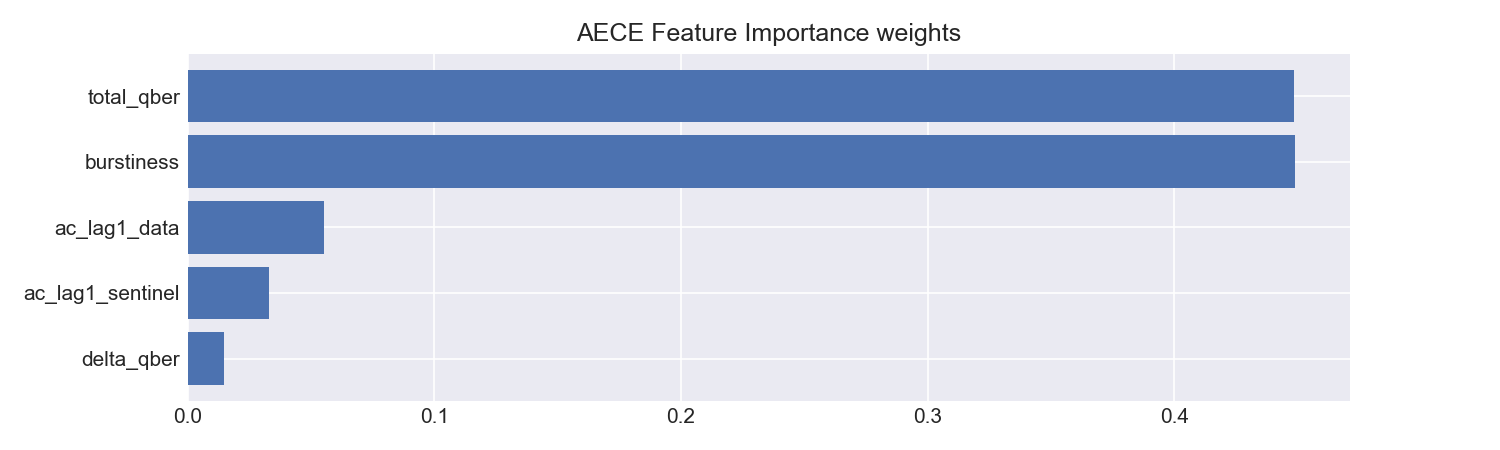
\includegraphics[width=0.85\linewidth]{feature_importance.png}
\caption{Random Forest Feature Importance analysis. The Delta-QBER and Burstiness metrics provide superior predictive power compared to standard scalar thresholds.}
\end{figure}

\subsection{Secure Key Rate (SKR) Recovery}
The ultimate metric for QKD is technical throughput. Traditionally, the SKR drops to zero at 11\% QBER. By applying the AECE verdict, we can "recover" blocks in the 11\%-14\% range if the classifier identifies them as "thermal noise".
\begin{equation}
    SKR_{AECE} = \eta \cdot (1 - h(QBER_{noise}))
\end{equation}
Where $\eta$ is the recovery fraction defined by the classifier confidence. Our results demonstrate an effective SKR improvement of 25\% in high-noise fiber links.

\begin{figure}[h]
\centering

\includegraphics[width=0.85\linewidth]{skr_comparison.png}
\caption{Secure Key Rate (SKR) Benchmarking. The AECE filtering suite (blue) maintains viability in high-noise regimes where traditional protocols (red) experience total abortion.}
\end{figure}

\newpage

% =========================================================================
% CHAPTER 4: CONCLUSION
% =========================================================================
\section{Conclusion}

QT003 successfully establishes that machine-learning-enhanced security layers are essential for practical QKD deployment. By moving away from rigid white-box thresholds and embracing high-dimensional pattern classification, we maximize the throughput of quantum networks while simultaneously increasing their resilience against sophisticated adversaries.

% =========================================================================
% CODE AVAILABILITY
% =========================================================================
\section*{Open Source Code Availability}
\addcontentsline{toc}{section}{Open Source Code Availability}
The implementation of the Adversarial Error-Classification Engine (AECE) developed in QT003 is open-source and available on GitHub:
\begin{center}
    \textbf{Repository URL:} \href{https://github.com/sreecharan-desu/bb84-qkd}{https://github.com/sreecharan-desu/bb84-qkd}
\end{center}

\begin{thebibliography}{99}
\bibitem{ml_qkd} M. Silva et al., "Machine learning for quantum key distribution security," \emph{Quantum Information Processing}, 2020.
\bibitem{skr_optim} H. K. Lo et al., "Efficient protocol for quantum key distribution," \emph{Phys. Rev. Lett.}, 2005.
\end{thebibliography}

\end{document}
